\chapter{Introduction}

\section{Human Genetics and the Genetics of Complex Traits}

A central goal of genetics is to understand the contribution of genetic variation to phenotypic variation.


\begin{figure}
\centering
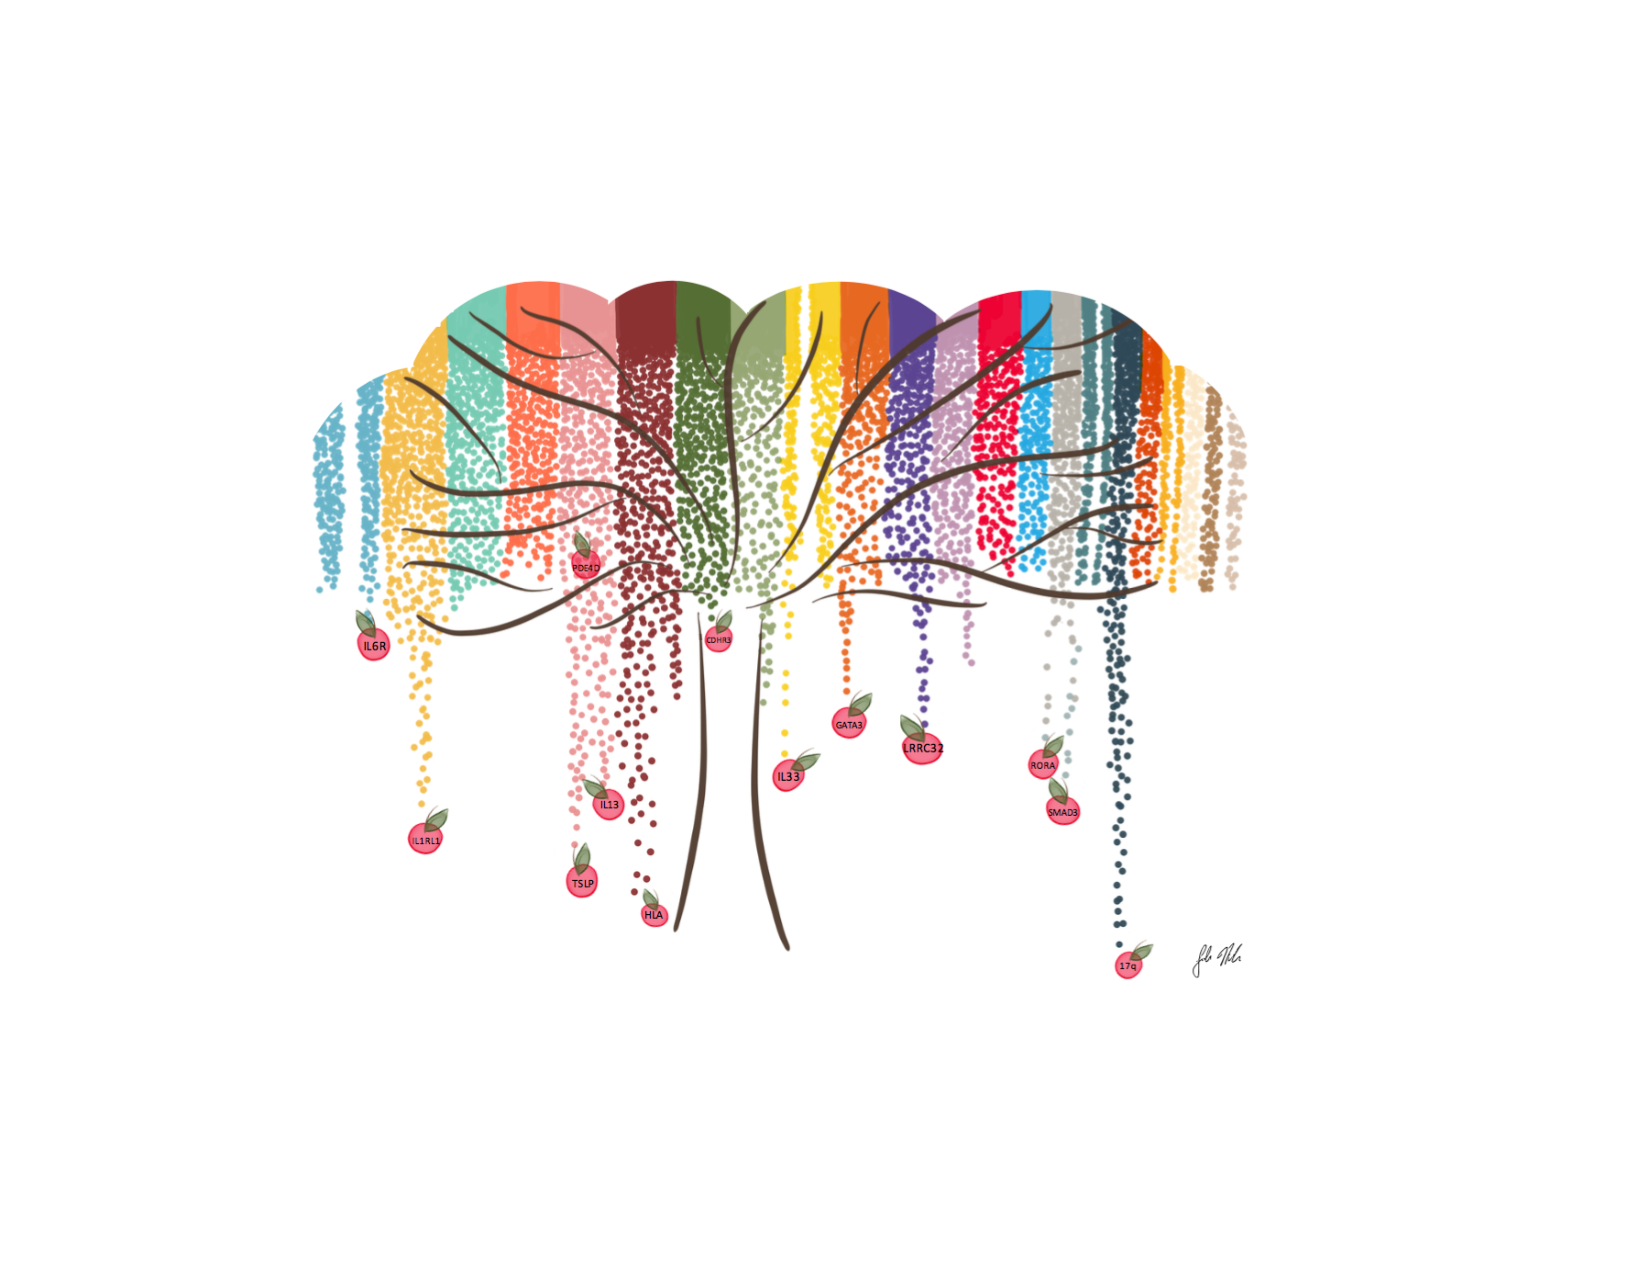
\includegraphics[width=5in]{img/ch01/fig-01-lowhangingfruit.pdf}
\caption[Low Hanging Fruit.]{\textbf{Asthma GWAS - low hanging fruit}}
\label{fig:lowhangingfruit}
\end{figure}


\section{On The Origin of Genomic Imprinting }

Genomic imprinting in its broadest sense suggests that a phenotype observed for a particular gene or genes depends on the sex of the parent from with the gamete containing that gene or genes originated \cite{Sapienza:1989vm}. It was said that a particular gene is imprinted if it results in a different phenotype when it is maternally inherited versus paternally inherited.

The first use of the term "imprinting" was used in reference to the recognition by the cell of of chromosomes in \textit{Sciara} \cite{Crouse:1960vc,Sapienza:1989vm}. "The "imprint" a chromosome bears is unrelated to the genic constitution of the chromosome and is determined only by the sex of the germ line through with the chromosome has been inherited." \cite{Crouse:1960vc} 

The preferential inactivation of the paternally-derived X chromosomes in mouse were the first demonstrations of a functional imprint in mammalian genomes \cite{Takagi:1975ua,Lyon:1984gh,Chandra:1975tb}. The first suggestion of imprinting on autosomes was by a deletion on mouse chromosome 17 that showed a different phenotype based on which parent the deletion was inherited from \cite{Johnson:1974uf,Johnson:1974kc}. The development of the pronuclear transplantation technique allowed for the creation of mice zygotes which contained only maternal or only paternal genetic contributions and provided evidence that the maternal and paternal genomes are not equal. The differential imprinting on the parental chromosomes prevented complete embryonic development in these mice with complete uniparental disomy \cite{Sapienza:1989vm,McGrath:1984ky}. 

Further experiments suggested that imprinting occurs during gametogenesis and is necessary for full term development; an egg with a male pronucleus developed to term, however, an egg with two female pronuclei (gynogenetic embryos) or two male pronuclei (androgenetic) developed poorly\cite{Surani1984,McGrath:1984ky}. Non-complementation in genetic crosses of translocated chromosomes provided a way to refine the imprinted regions of the genome\cite{Cattanach:1985hu}. 

Genetic characterization of Prader-Willi syndrome (PWS) was the first human genetic disease to be associated with maternal heterodisomy of chromosome 15q11-13\cite{Nicholls:vh}. It suggested that  clinical phenotype of PWS arises from the absence of paternal contribution of 15q11-13 as opposed to a specific genetic mutation. Conversely the absence of maternal contribution to the same region should result in Angelman syndrome (AS)\cite{Nicholls:vh,Reik:1989el}. This provided more evident that at "imprinted" regions the functional differences depend on the sex of the transmitting parent and genetic input from both parents are required for normal human development\cite{Nicholls:vh}.

A rare disease, PWS affects between 1 in 10,000 and 30,000 people. PWS arises from loss of paternal genetic contribution at 15q11-13, mostly by chance mutation but also through uniparental disomy, sporadic mutations, chromosome translocations, and gene deletions. (wiki). On the other side of the spectrum, AS is also rare, affecting between 1 in 12,000 and 20,000 people and is caused by the loss of the normal maternal contribution at 15q11-13. (wiki) Various other human imprinted syndromes due to loss or gain of expression of imprinted genes have been characterized (Table \ref{tab:imprinteddisease}). \cite{Peters2014}

\begin{table}
\centering
\begin{tabular}{@{}llll@{}}
\toprule Abbr. & Name & Description & Gram staining* \\ \midrule none
& control & Mock infection & N/A \\ Rv & MTB H37Rv & A common
laboratory strain of MTB & acid-fast \\ Rv+ & heat-inactivated MTB
H37Rv & Dead MTB H37Rv & acid-fast \\ GC & MTB GC1237 & More virulent
strain of MTB & acid-fast \\ BCG & bacillus Calmette-Gu\'{e}rin &
Vaccine (attenuated \emph{M. bovis}) & acid-fast \\ Smeg &
\emph{Mycobacterium smegmatis} & Non-pathogenic mycobacterium &
acid-fast \\ Yers & \emph{Yersinia pseudotuberculosis} & Facultative
intracellular pathogen & Negative \\ Salm & \emph{Salmonella
  typhimurium} & Facultative intracellular pathogen & Negative
\\ Staph & \emph{Staphylococcus epidermidis} & Extracellular pathogen
& Positive \\ \bottomrule
\end{tabular}
\caption[Description of bacteria.]{\textbf{Description of bacteria.}
  *Mycobacteria are unable to be gram stained due to the low
  permeability of their cell walls. They are more closely related
  evolutionarily to gram-positive bacteria than
  gram-negative. However, their thick cells walls share features of
  gram-negative bacteria, e.g. a ``pseudoperiplasm'' similar to the
  gram-negative periplasm.}
\label{tab:imprinteddisease}
\end{table}


\section{The Search for Parent of Origin Effects}


